\documentclass{beamer}

\mode<presentation>
{
  \useinnertheme[shadow=true]{rounded} % default from Warsaw theme
  \useoutertheme[subsection=false]{miniframes}

  \usecolortheme{orchid} % default from Warsaw theme
  \usecolortheme{whale} % default from Warsaw theme
  \usecolortheme{beaver} % this overrides both orchid and whale, as far as I~see, but keep them for safety

  % these override \usecolortheme above
  \setbeamercolor{frametitle}{bg=,fg=darkred!80!black}
  \setbeamercolor{frametitle right}{bg=}
  \setbeamercolor{palette tertiary}{fg=black,bg=gray!15!white}

  \usefonttheme[onlylarge]{structurebold}
  \setbeamerfont{block title}{size={}} % default from Warsaw theme
  \setbeamerfont{frametitle}{series=\bfseries} % probably taken care of by structurebold anyway, but keep in case useful for the future

  \setbeamercovered{transparent}
}

\usepackage[polish]{babel}
\usepackage[utf8]{inputenc}
\usepackage{times}
\usepackage[T1]{fontenc}

\title{Komponowanie shaderów w~X3D}
\author[Michalis Kamburelis]{Michalis Kamburelis \\ \texttt{michalis.kambi@gmail.com}}
\date{31 maja 2011}

\AtBeginSection[]
{
  \begin{frame}<beamer>{Plan}
    \tableofcontents[currentsection,currentsubsection]
  \end{frame}
}

\begin{document}

{
  % logo on title page
  \pgfdeclareimage[height=2cm]{ii-and-kambivrml}{ii-and-kambivrml}
  \logo{\pgfuseimage{ii-and-kambivrml}}
  \begin{frame}
    \titlepage
  \end{frame}
}

\begin{frame}{Plan}
  \tableofcontents
  % You might wish to add the option [pausesections]
\end{frame}

\section{Wstęp}

\begin{frame}{Wstęp}
Jak tworzyć i~łączyć efekty graficzne oparte na~shaderach.

\begin{itemize}
  \item Rozszerzenie dwóch zintegrowanych ze sobą języków (X3D i~GLSL).
  \item Praktyczne, implementowalne (100\% skończona
    i~przetestowana implementacja open-source).
\end{itemize}
\end{frame}

\begin{frame}{Proste i~działa}

Proste, ale nikt inny tego jeszcze nie zrobił :)

\begin{itemize}
  \item Przynajmniej nie bez wymyślania zupełnie nowego języka pisania shaderów
    (Spark, Sh). Ale nowe języki nie zdobywają popularności,
    bo zazwyczaj wymagają przepisania całego renderowania.
    Nasz pomysł to eleganckie rozszerzenie GLSL i~X3D.
    % glsl - (który jest podstawą OpenGL, więc znają go wszyscy
\end{itemize}

Działa świetnie :) Istotnie różne algorytmy na~shaderach stają się łatwe,
i~to do~,,prawdziwej'' implementacji (która, raz zrobiona,
musi być użyteczna na~różnych modelach).
Będą ładne obrazki.

    % Istotnie pozwalam na~programowanie i~łączenie efektów
    % za~pomocą shaderów w~bardzo wygodny sposób.
    %  IMHO dopiero teraz GLSL jest użyteczny dla~autorów.

\end{frame}

\section{Co to jest X3D, co to są shadery}

\begin{frame}[fragile]{X3D}

\begin{itemize}
  \item \textbf{Extensible 3D}: język do~opisu światów 3D.
  \item Otwarty (pełne specyfikacje na~\texttt{http://www.web3d.org/}), popularny standard.
  \item Łatwo wyrazić wszystkie typowe elementy świata 3D.
  \item Drzewo węzłów w~wielu prostych przypadkach.
    Ale ogólnie skierowany graf węzłów, z~możliwymi cyklami.
  \item Każdy węzeł ma pola, niektóre pola mogą zawierać węzły-dzieci.
\end{itemize}

\begin{exampleblock}{Przykład}
\begin{semiverbatim}
\#X3D V3.2 utf8
PROFILE Interchange
Shape \{
  geometry Sphere \{ radius 2 \}
\}
\end{semiverbatim}
\end{exampleblock}
\end{frame}

\begin{frame}[fragile]{X3D - XML}

Alternatywna wersja:

\begin{exampleblock}{Przykład kodowania XML}
\begin{semiverbatim}
...
<X3D version="3.2" profile="Interchange" ...>
  <Scene>
    <Shape>
      <Sphere radius="2" />
    </Shape>
  </Scene>
</X3D>
\end{semiverbatim}
\end{exampleblock}

\end{frame}

\begin{frame}{X3D jako język programowania}

Kilka elementów które czynią X3D bardziej interesującym,
jako ,,deklaratywny język programowania'':

\begin{itemize}
  \item DEF/USE: referencje, dla~wszystkich węzłów.
  \item Mechanizm zdarzeń: wysyłanie i~reagowanie na~zdarzenia.
    Deklaratywny odpowiednik wywołania metody obiektu.
    Np.~otwórz drzwi kiedy user kliknie na~klamkę.
  \item Prototypy: można definiować nowe, pełnowartościowe,
    węzły jako kombinację istniejących.
  \item Skrypty: integracja z~innymi językami (np. JavaScript) łatwa.
    Skrypt pozostaje ,,black boxem'' dla~X3D, jednocześnie w~samym
    X3D definiujemy precyzyjnie do~czego skrypt ma a do~czego nie ma dostępu.
     %  np.~JavaScript. U mnie --- z~własnym prostym językiem skryptowym
     % oraz ze skompilowanym kodem w~ObjectPascalu.
     % Więcej nowinek w~vrml\_engine\_doc, sekcja "advanced features".
\end{itemize}
\end{frame}

\begin{frame}{Shadery}
Shadery:
\begin{itemize}
  \item Języki do~cieniowania obiektów 3D. Zaprogramuj pracę per-vertex,
    pozwól na~rasteryzację, zaprogramuj pracę per-pixel.
    % Chociaż przy pomocy pewnych sztuczek (tekstury oparte na~float,
    % render to textury) można je wykorzystać do~ogólnych obliczeń,
    % obecnie do~ogólnych obliczeń wygodniejsze są CUDA/OpenCL
    % (google.com/q=gpgpu).
    % Można próbować
    % geom shader
  \item Nas interesują shadery na~GPU, czyli do~renderowania w~czasie
    rzeczywistym. GLSL (OpenGL), Cg (NVidia: dla~OpenGL lub~Direct 3D),
    HLSL (Direct 3D).
  \item Naturalnie, X3D posiada węzły do~definiowania shaderów.
\end{itemize}
\end{frame}

\begin{frame}[fragile]
\begin{exampleblock}{Przykład X3D + GLSL}
\begin{semiverbatim}
\#X3D V3.2 utf8
PROFILE Interchange
Shape \{
  appearance Appearance \{
    shaders ComposedShader \{
      language "GLSL"
      parts ShaderPart \{
        type "FRAGMENT"
        url "data:text/plain,
        \textbf{void main(void)}
        \textbf{\{}
          \textbf{gl\_FragColor = vec4(1.0,0.0,0.0,1.0);}
        \textbf{\}}" \} \} \}
  geometry Sphere \{ radius 2 \}
\}
\end{semiverbatim}
\end{exampleblock}
\end{frame}

\begin{frame}{Shader zastępuje domyślne obliczenia}

\begin{itemize}
  %  \item + Wybiera pierwszy obsługiwany shader.
  %% \item + Można łatwo przekazać do~shadera wartości uniform (per-object)
  %%   albo attribute (per-vertex). Np.~przekaż aktualny czas
  %%    to shadera.
  \item + Łatwa implementacja dla~renderera, bo właśnie tak działają GPU,
    na~to pozwala OpenGL etc.
  \item - \textbf{Trudne implementowanie własnych shaderów}.
    Zanim zaczniesz pisać swój efekt, najpierw odtwórz algorytm
    standardowego renderowania.
    Możesz skopiować kod wygenerowany przez renderer,
    i~zorientować się gdzie dodać swoje modyfikacje, ale...
  \item - \textbf{Powstają shadery 1-razowego użytku}.
    Konkretny kod shadera przywiązuje Cię do~wielu ustawień sceny
    (ile, jakie tekstury, światła etc.).
    Ogólny shader (uwzględniający wszystkie możliwości) nie jest możliwy,
    chociażby dlatego że nie ma będzie działał szybko.
  \item - \textbf{Wszystkie efekty w~jednym worku}.
    Usuwanie / dodawanie efektu oznacza ostrożne wstawianie logiki
    do~istniejącego (dużego) kodu.
\end{itemize}
\end{frame}

\section[Nasz pomysł]{Nasz pomysł: komponowanie shaderów w X3D}

\begin{frame}{Dlaczego}
\begin{itemize}
  \item Chcielibyśmy intensywnie używać shaderów. Każda właściwość 3D powinna
    być programowalna --- po to stworzono shadery.

  \item Ale tradycyjne podejście, ,,napisz shader który robi wszystko'',
    uniemożliwia to. Zaprogramowanie najmniejszej zmiany (np. przefiltruj
    światło przez szablon) wymaga zatroszczenia się o~algorytm naokoło.

  \item Wolimy programować efekty które rozszerzają/modyfikują
    istniejące zachowanie.
\end{itemize}
\end{frame}

\begin{frame}{Rozwiązanie}

\begin{block}{Pomysł 1}
Prosty w~użyciu mechanizm do~definiowania i~używania
,,gniazd'' (plugs) --- miejsc gdzie można dodać własne obliczenia.
Żeby użyć gniazda o~nazwie \texttt{texture\_apply},
zdefiniuj funkcję o~magicznej nazwie \texttt{PLUG\_texture\_apply}
w~nowym węźle \texttt{Effect}.
\end{block}

\begin{itemize}
  \item Zachowujemy pełną siłę języka shaderów (GLSL).
    %% - You still have the full power of shading language like GLSL
    %%   (we do~not hide it from you, we do~not invent any new language
    %%   for writing shaders, and implementation doesn't have to do~any
    %%   difficult operations to process your shading language code).
  \item Implementacja w~rendererze łatwa: rozszerzamy istniejący język.
  \item Implementacja efektów łatwa: zaczynamy od razu pisać nasz algorytm,
    wskazujemy tylko gdzie wstawić odpowiednie elementy.
  \item Efekty reusable: wstawiane w~wewnętrzny shader, wygenerowany
    znając tekstury, oświetlenie etc.
  \item Efekty można łączyć: wiele efektów może używać tych samych gniazd.
\end{itemize}
\end{frame}

\begin{frame}[fragile]
\begin{exampleblock}{Przykład naszego efektu}
\begin{semiverbatim}
# w środku Appearance z poprzedniego przykładu:
effects Effect \{
  language "GLSL"
  parts EffectPart \{
    type "FRAGMENT"
    url "data:text/plain,
\textbf{    void PLUG\_texture\_apply(}
\textbf{      inout vec4 fragment\_color,}
\textbf{      const in vec3 normal)}
\textbf{    \{}
\textbf{      fragment\_color.rgb *= 2.0;}
\textbf{    \}}"
  \}
\}
\end{semiverbatim}
\end{exampleblock}
\end{frame}

\renewcommand*{\figurename}{Obraz}

\begin{frame}{Szczegóły}
\begin{itemize}
  \item Nowy węzeł \texttt{Effect}: wybierz język shaderów.
  \item Nowy węzeł \texttt{EffectPart}: wybierz typ (vertex, pixel, etc.).
  \item Można definiować własne uniform w~\texttt{Effect}, np.~przekazać
    teksturę albo czas (\texttt{TimeSensor.time} z~X3D) do~efektu.
    % jak ComposedShader
  \item Wszystkie efekty będą dodane do~bazowego shadera. (Upraszczając.)
  \item Stary \texttt{ComposedShader} modyfikuje bazowy shader.
    W~ten sposób stary \texttt{ComposedShader} też jest lepszy:
    może współpracować z~wewnętrznymi efektami (shadow maps),
    i~efektami użytkownika (z węzłów \texttt{Effect}).
\end{itemize}
\end{frame}

\begin{frame}{Przykład - łączenie prostych efektów}
\begin{figure}
  \centering
  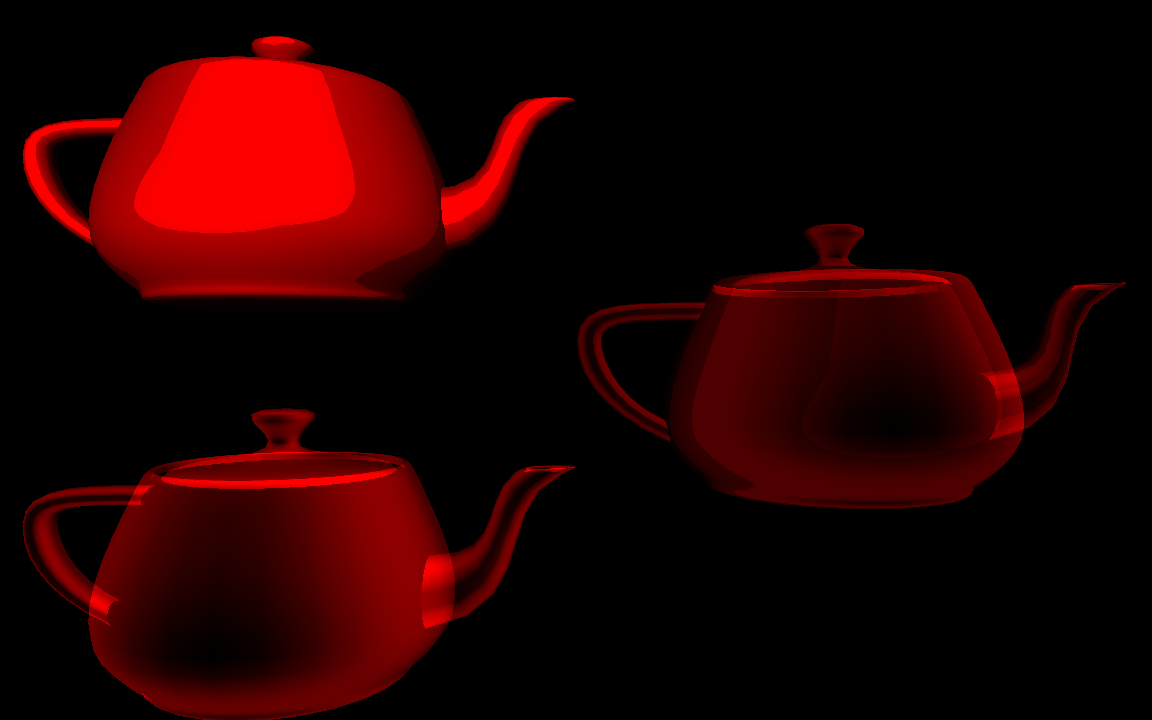
\includegraphics[width=3.0in]{../fresnel_and_toon}
  \caption{Połączenie dwóch prostych efektów Fresnela i~cieniowania kreskówkowego}
\end{figure}

Kod: \texttt{demo\_models/compositing\_shaders/\\fresnel\_and\_toon.x3dv}

  %% : show the X3D source:
  %%   I~can just say: "this is a list of effects you should use:
  %%   this one, and this one. Now make it happen."
  %%   And both effects are applied.
\end{frame}

\begin{frame}{Wewnętrzne efekty}
Możemy zaimplementować wewnętrzne efekty w~podobny sposób.

\begin{itemize}
  \item Shadow maps: filtruj odpowiednie źródło światła,
  \item Klasyczny Bump mapping: zmień wektor normalny na~podstawie tekstury,
  \item Mgła: wymieszaj końcowy kolor pixela z~kolorem mgły.
\end{itemize}

\begin{figure}
  \centering
  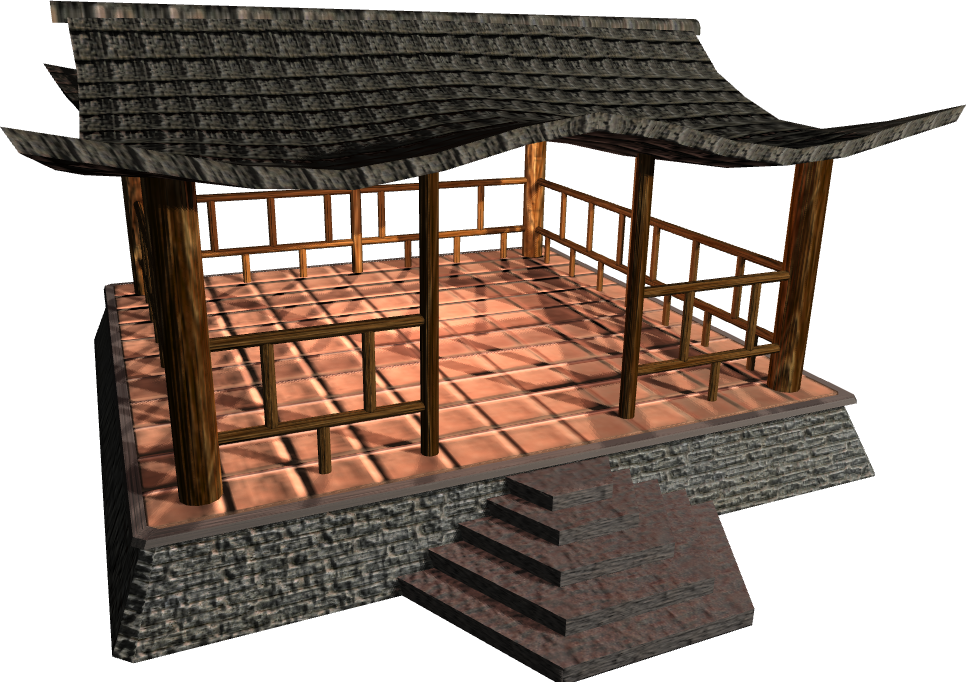
\includegraphics[width=2in]{../rhan_shrine_5_everything}
  \caption{Połączenie dwóch shadow maps i~bump mapping}
\end{figure}
\end{frame}

\begin{frame}{Efekty dla~źródeł światła}
\begin{block}{Pomysł 2}
Efekty można dodawać nie tylko do~widocznych obiektów 3D.
Można zdefiniować światło które ma specyficzny kształt, równanie itp.,
i używać go wielokrotnie jako pełnowartościowe światło w~X3D.
\end{block}

\begin{figure}
  \centering
  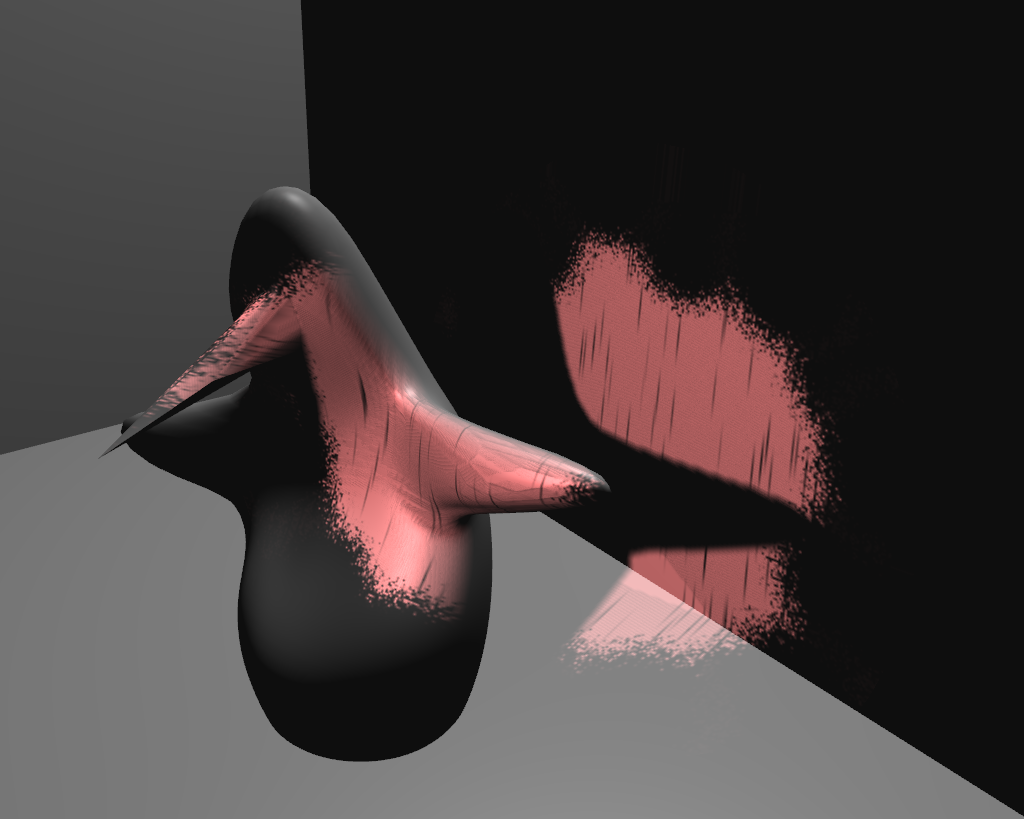
\includegraphics[width=1.8in]{../fancy_light_spot_shape}
  \caption{Światło filtrowane przez teksturę. Rzuca poprawny cień, współpracuje z~bump mapping (czego nie mamy przy prostym rzutowaniu tekstury na~ścianę).}
\end{figure}
\end{frame}

\begin{frame}[fragile]{Efekty tekstur}
Tekstury można modyfikować przy użyciu efektów. Tekstury mają mnóstwo
zastosowań (to po prostu macierz, zazwyczaj 2D lub~3D), więc wiele nowych
możliwości.

\vspace{0.1in}

Np.~zaburz istniejącą teksturę losowym szumem, albo wybierz slice tekstury 3D.
\end{frame}

\begin{frame}[fragile]{Proceduralne tekstury na~GPU}
Proceduralna tekstura to po prostu funkcja 2D lub~3D $\rightarrow$
kolor, wektor normalny, i~inne.

\vspace{0.1in}

Tworzenie ich zawsze było łatwe, ale tradycyjne metody miały wadę:
ponieważ nie jest to tekstura dla~renderera, znikały możliwości wygodnego
generowania i~przypisywania współrzędnych tekstury. Rozwiązujemy to przez
\texttt{ShaderTexture}.

\begin{center}
\begin{columns}[T]
  \begin{column}{1in}
    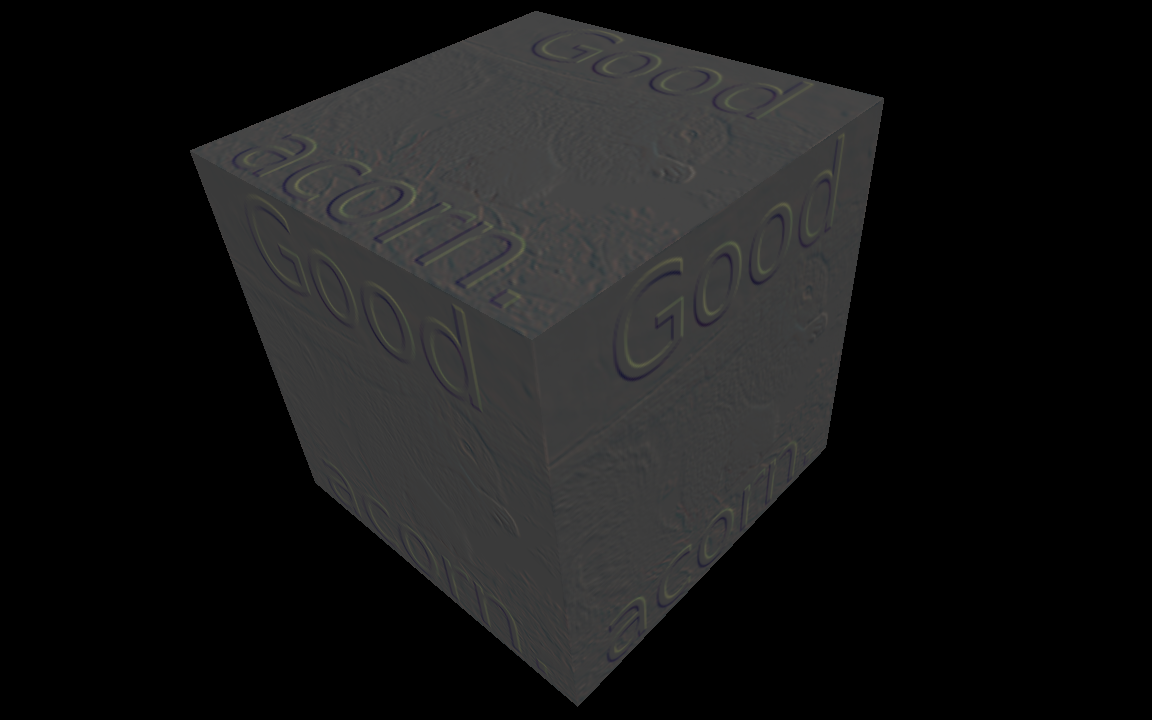
\includegraphics[width=1.3in]{../shader_texture_edge_detection}
  \end{column}
  \begin{column}{1in}
    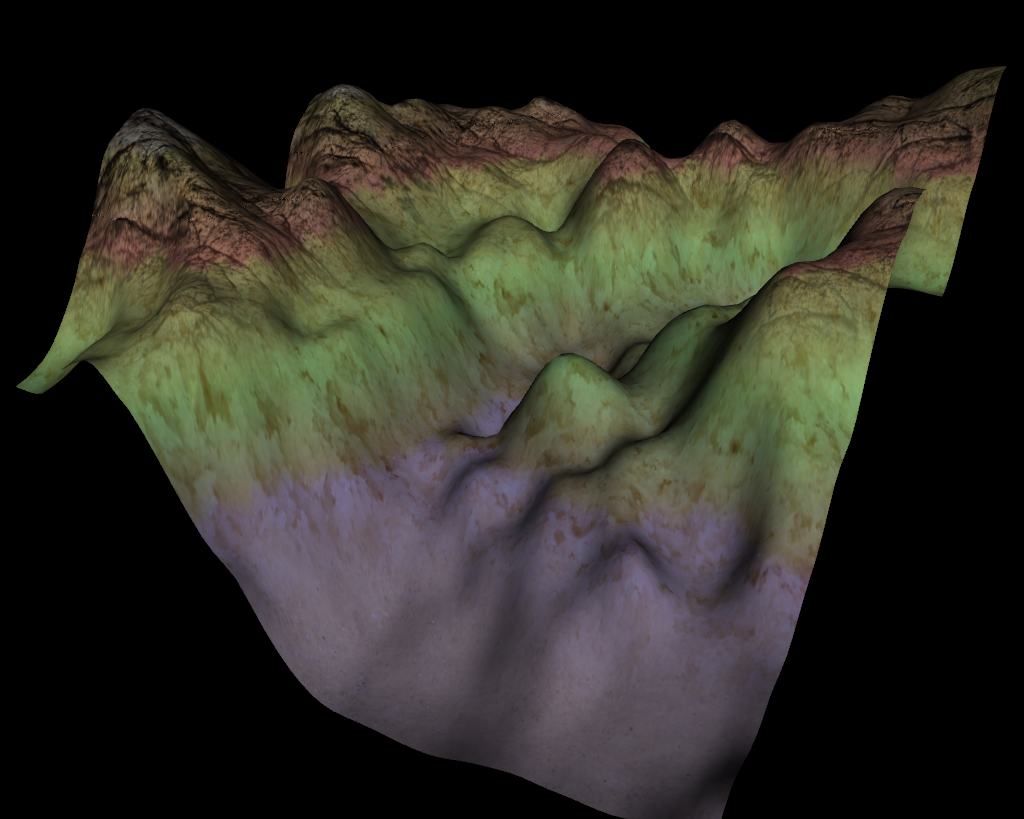
\includegraphics[width=1.3in]{../terrain}
  \end{column}
  \begin{column}{1in}
    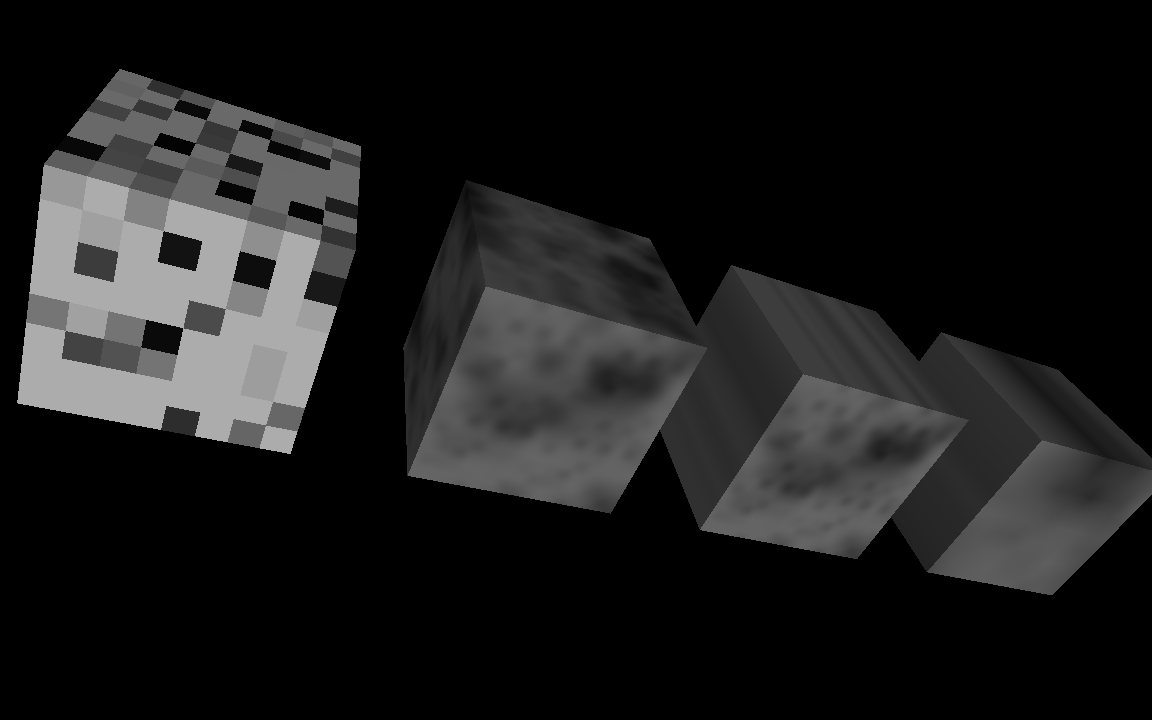
\includegraphics[width=1.3in]{../noise}
  \end{column}
\end{columns}
\end{center}

\end{frame}

\begin{frame}{Efekty działające na~grupę}
%Naturalne rozszerzenie.

\begin{figure}
  \centering
  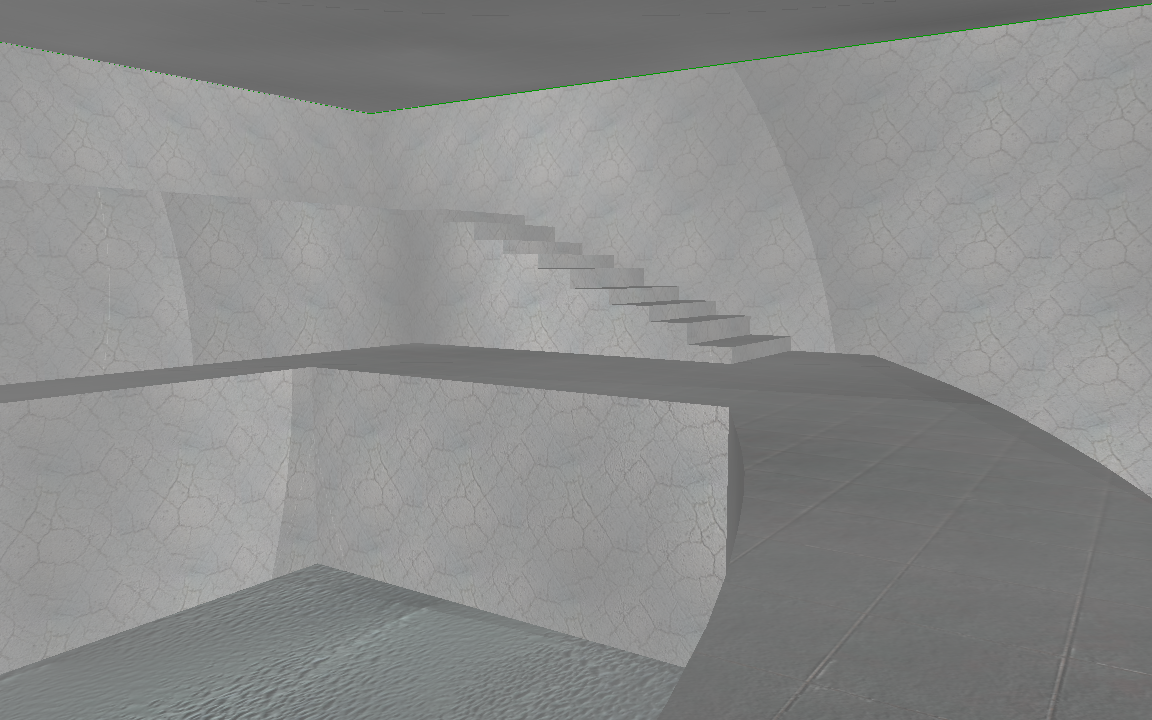
\includegraphics[width=3in]{../volumetric_animated_fog_all}
  \caption{Kłębiasta, ruchoma mgła (sauna).}
\end{figure}

Kod: \texttt{demo\_models/compositing\_shaders/\\volumetric\_animated\_fog.x3dv}\\
\textbf{Krótki i~działa na~dowolnym modelu 3D!}

% Unline other implementation.)
% Turn on/off fog.

\end{frame}

\begin{frame}{Definiuj własne gniazda}
Cały system polega na tym że własne gniazda można definiować łatwo:
\begin{itemize}
  \item Bazowy shader, i \textbf{każdy efekt}, może definiować gniazda
    do~użycia przez następne efekty.\\
    Trywialne: magiczny komentarz \texttt{/* PLUG: ... */}.
  \item Magicznego komentarza można użyć wielokrotnie (żeby pozwolić
    na loop unrolling w shaderach).
  \item Magiczny komentarz \texttt{/* PLUG-DECLARATION */}
    (przydatny żeby można było zadeklarować wyższą wersję GLSL).
  \item Elegancko korzystamy z \textit{separate compilation units} GLSL.
  \item Pomysł przenośny do innych języków shaderów.
  \item Dobrze dobrany domyślny zestaw gniazd, see linki na końcu i przykłady.
    Wbrew pozorom, nie trzeba 100 gniazd --- istnieje kilka uniwersalnych
    gniazd które zaspokajają 90\% potrzeb.
\end{itemize}
\end{frame}

\begin{frame}{Przykłady końcowe - woda}
\begin{figure}
  \centering
  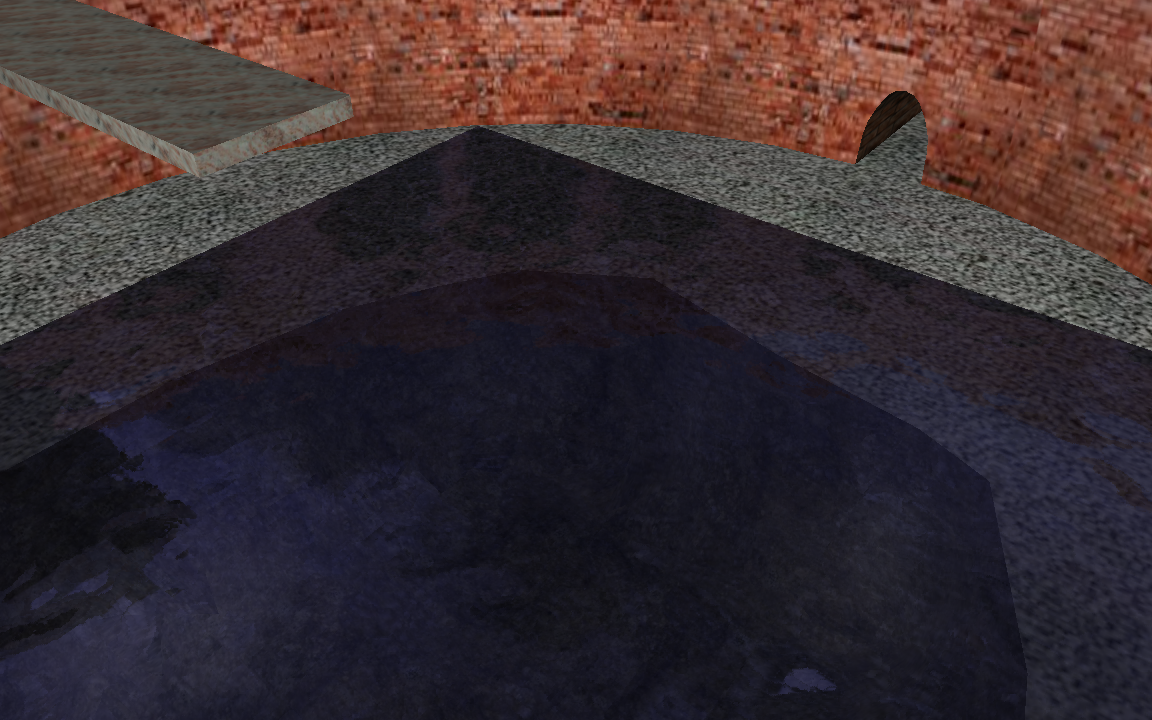
\includegraphics[width=3.5in]{../water_shaders_3}
  \caption{Woda, połączenie kilku efektów: generuj wektory normalne, transformuj je do~eye space, połącz z~reflection + refraction}
\end{figure}
\end{frame}

\begin{frame}
\begin{figure}
  \centering
  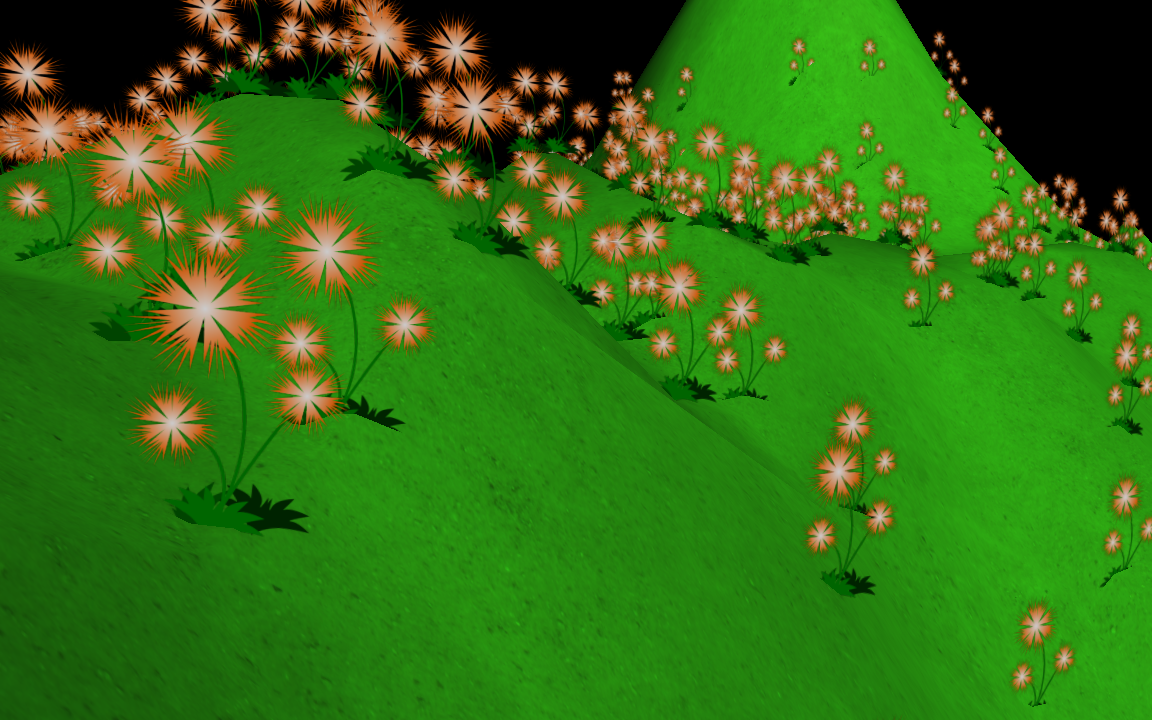
\includegraphics[width=3.5in]{../flowers}
  \caption{Animowane kwiatki: transformacja w~object space zmieniana przez shader.}
\end{figure}
\end{frame}

\section{Pytania?}

\begin{frame}[t]

\begin{center}
{\small
Wszystko jest zaimplementowane, open-source (LGPL), w~moim silniku:\\
{\color{blue} \textbf{\texttt{http://vrmlengine.sourceforge.net/}}}\\
Instrukcje jak pobrać i~oglądać przykładowe modele dotyczące komponowania
shaderów:\\
{\color{blue} \textbf{\texttt{http://vrmlengine.sourceforge.net/\\
compositing\_shaders.php}}}}
\end{center}

\vspace{0.25in}

\begin{center}
{\Large Dziękuję za~uwagę!}
\end{center}

%\vspace{0.1in}

\begin{center}
{\Huge \alert{Pytania?}}
\end{center}

\end{frame}

\end{document}
